\documentclass{beamer}

%\usetheme[framenumber,totalframenumber]{UniversiteitGent}
%\usetheme[faculty=di,framenumber,totalframenumber]{UniversiteitGent}
%\usetheme[faculty=we,usecolors,framenumber,totalframenumber]{UniversiteitGent}
%\usetheme[language=english,framenumber,totalframenumber]{AlleghenyCollege}
\usetheme{AnnArbor}
\usecolortheme{dove}

\title{CMPSC 390 \\ Decentralization}
\author{Janyl Jumadinova \\ $ $ \\ Credit: Authors of ``Bitcoin and Cryptocurrency Technologies"}
\date{January 25, 2021}

\long\def\omitit#1{}

\usepackage{hyperref}

\begin{document}

\begin{frame}
  \titlepage
\end{frame}

%%%%%%%%%%%% Slide %%%%%%%%%%%%%%%%%%%%%%%%%%%%%%%%%%%%%%%%%%%%%%%%%%%
\begin{frame}
  \frametitle{Decentralization in Bitcoin}
	\begin{enumerate}
		\item \textbf{Who maintains the ledger?}
		\item \textbf{Who has authority over which transactions are valid?}
		\item \textbf{Who creates new bitcoins?}
		\item Who determines how the rules of the system change?
		\item How do bitcoins acquire exchange value?
	\end{enumerate}
\end{frame}
%%%%%%%%%%%% Slide %%%%%%%%%%%%%%%%%%%%%%%%%%%%%%%%%%%%%%%%%%%%%%%%%%%
\begin{frame}
  \frametitle{Decentralization in Bitcoin}
  
  \begin{block}{\textbf{Peer-to-peer:}}
  Open to anyone, low barrier to entry.
   \end{block}
 	
     \begin{block}{\textbf{Mining:}}
  Open to anyone, but inevitable concentration of power
    often seen as undesirable.
 	\end{block}
 	
     \begin{block}{\textbf{Updates to software:}}
  Core developers trusted by community, have great power.
 	\end{block} 		
\end{frame}
%%%%%%%%%%%% Slide %%%%%%%%%%%%%%%%%%%%%%%%%%%%%%%%%%%%%%%%%%%%%%%%%%%
\begin{frame}
  \frametitle{Distributed Consensus}

     \begin{block}{\textcolor{red}{The protocol terminates and all correct nodes decide on the same value.}}
 	\end{block} 

     This value must have been proposed by some correct node.
\end{frame}
%%%%%%%%%%%% Slide %%%%%%%%%%%%%%%%%%%%%%%%%%%%%%%%%%%%%%%%%%%%%%%%%%%
\begin{frame}
  \frametitle{How consensus \emph{could} work in Bitcoin}
  
At any given time:

\begin{itemize}
	\item All nodes have a sequence of blocks of transactions they have reached consensus on.
	\item Each node has a set of outstanding transactions it has heard about.
\end{itemize}
\pause
	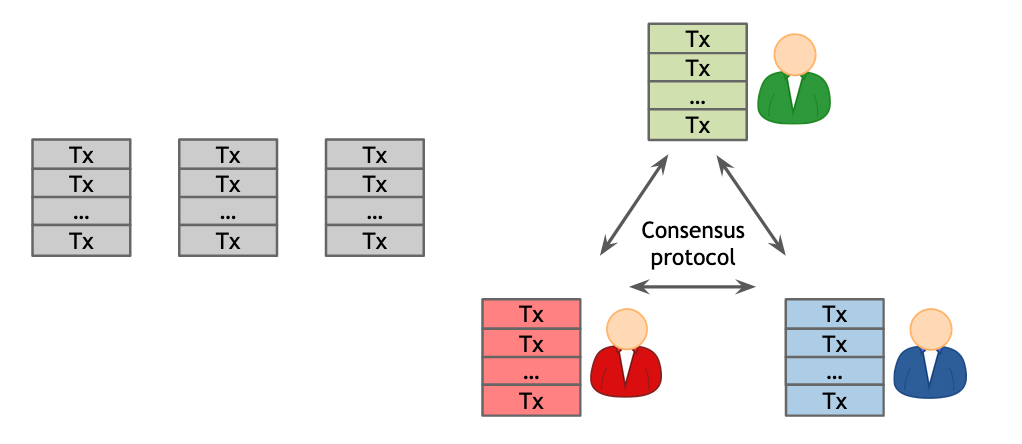
\includegraphics[scale=0.5]{consensus}
\end{frame}
%%%%%%%%%%%% Slide %%%%%%%%%%%%%%%%%%%%%%%%%%%%%%%%%%%%%%%%%%%%%%%%%%%
\begin{frame}
  \frametitle{Consensus is hard}
  \begin{itemize}
  	\item Nodes may crash.
	\item Nodes may be malicious. \pause
	\item Network is imperfect:
	\begin{itemize}
		\item Not all pairs of nodes connected.
		\item Faults in network.
		\item Latency.
	\end{itemize}
  \end{itemize}
\end{frame}
%%%%%%%%%%%% Slide %%%%%%%%%%%%%%%%%%%%%%%%%%%%%%%%%%%%%%%%%%%%%%%%%%%
\begin{frame}
  \frametitle{Bitcoin Consensus}
 
	\begin{itemize}
		\item Bitcoin consensus works better in practice than in theory.
		\item Theory is still catching up. \pause
		\item But theory is important, can help predict unforeseen attacks.
	\end{itemize}

\end{frame}

%%%%%%%%%%%% Slide %%%%%%%%%%%%%%%%%%%%%%%%%%%%%%%%%%%%%%%%%%%%%%%%%%%
\begin{frame}[fragile]
  \frametitle{Bitcoin Consensus}
 \emph{ Introduces incentives}
	\begin{itemize}
		\item Possible because it is a currency!
	\end{itemize}

	\pause
	\emph{Embraces randomness:}

	\begin{itemize}
		\item Does away with the notion of a specific end-point.
		\item Consensus happens over long time scales - about one hour.
	\end{itemize}
\end{frame}
%%%%%%%%%%%% Slide %%%%%%%%%%%%%%%%%%%%%%%%%%%%%%%%%%%%%%%%%%%%%%%%%%%
\begin{frame}
  \frametitle{Implicit Consensus}

	\begin{itemize}
		\item In each round, random node is picked. \pause
		\item This node proposes the next block in the chain. \pause
		\item Other nodes implicitly accept/reject this block:
		\begin{itemize}
			\item by either extending it,
			\item or ignoring it and extending chain from earlier block.
		\end{itemize}
	\end{itemize}
	\pause
\emph{Every block contains hash of the block it extends.}

\end{frame}
%%%%%%%%%%%% Slide %%%%%%%%%%%%%%%%%%%%%%%%%%%%%%%%%%%%%%%%%%%%%%%%%%%
\begin{frame}
  \frametitle{Consensus algorithm (simplified)}
	\begin{enumerate}
		\item New transactions are broadcast to all nodes. \pause
		\item Each node collects new transactions into a block. \pause
		\item In each round a \emph{random} node gets to broadcast its block. \pause
		\item Other nodes accept the block only if all transactions in it are valid (unspent, valid signatures). \pause
		\item Nodes express their acceptance of the block by including its hash in the next block they create.
	\end{enumerate}
\end{frame}
%%%%%%%%%%%% Slide %%%%%%%%%%%%%%%%%%%%%%%%%%%%%%%%%%%%%%%%%%%%%%%%%%%
\begin{frame}
  \frametitle{Malicious node?}
  \centering
	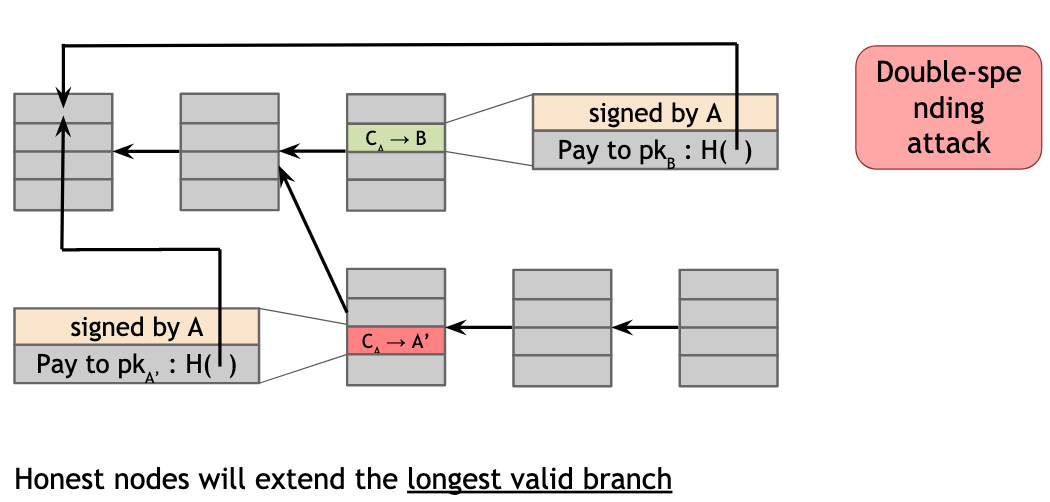
\includegraphics[scale=0.6]{attack}
\end{frame}
%%%%%%%%%%%% Slide %%%%%%%%%%%%%%%%%%%%%%%%%%%%%%%%%%%%%%%%%%%%%%%%%%%
\begin{frame}
  \frametitle{From merchant's point of view}
  \centering
	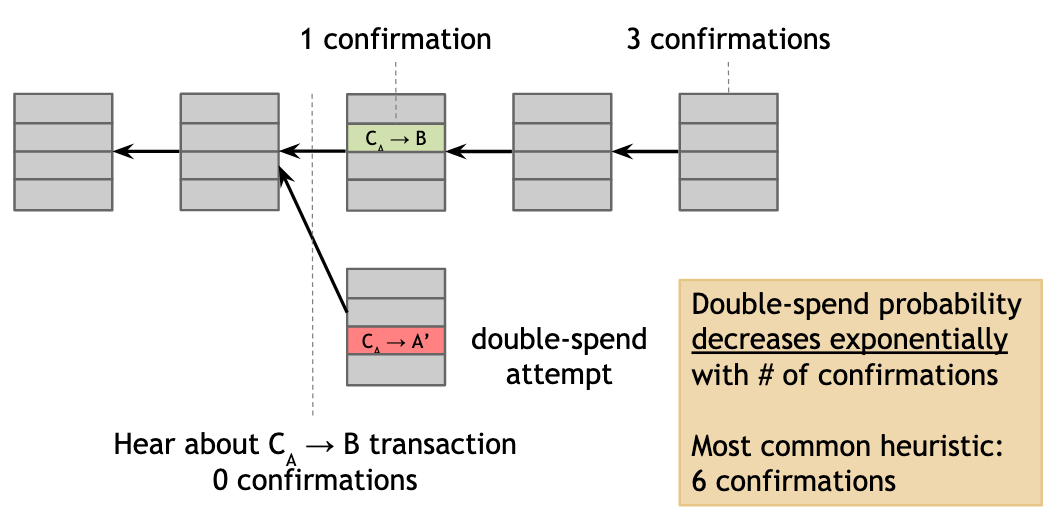
\includegraphics[scale=0.6]{double_spend}
\end{frame}
%%%%%%%%%%%% Slide %%%%%%%%%%%%%%%%%%%%%%%%%%%%%%%%%%%%%%%%%%%%%%%%%%%
\begin{frame}
  \frametitle{Summary}
	\begin{itemize}
		\item Protection against invalid transactions is cryptographic, 
but enforced by consensus.
		\item Protection against double-spending is purely by consensus.
		\item You are never 100\% certain a transaction is in consensus branch. Guarantee is probabilistic.
	\end{itemize}
\end{frame}
%%%%%%%%%%%% Slide %%%%%%%%%%%%%%%%%%%%%%%%%%%%%%%%%%%%%%%%%%%%%%%%%%%
\begin{frame}
  \frametitle{Assumption of honesty is problematic}
Can we give nodes incentives for behaving honestly?

	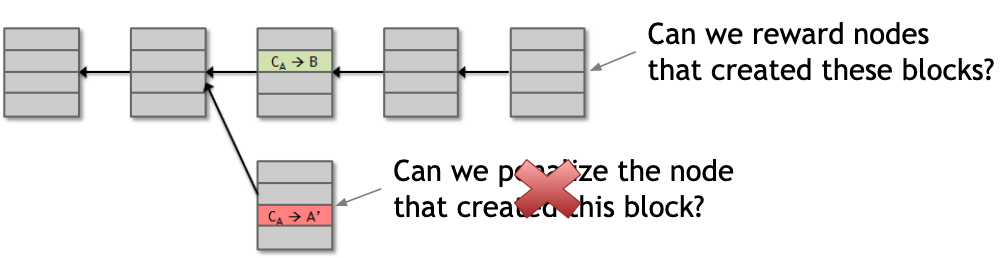
\includegraphics[scale=0.7]{incentives}
	
	\pause
	
Everything so far is just a distributed consensus protocol ... \pause
but now we utilize the fact that the currency has value.

\end{frame}
%%%%%%%%%%%% Slide %%%%%%%%%%%%%%%%%%%%%%%%%%%%%%%%%%%%%%%%%%%%%%%%%%%
\begin{frame}
  \frametitle{Incentive 1: block reward}
	Creator of block gets to: 
	\begin{itemize}
		\item include \emph{special coin-creation transaction} in the block,
		\item choose recipient address of this transaction.
	\end{itemize}
	\pause
	Value is fixed, halves every 4 years. \\ $ $ \\
	\pause
	
	\emph{Block creator gets to ``collect'' the reward only if the block ends up on long-term consensus branch!}
\end{frame}
%%%%%%%%%%%% Slide %%%%%%%%%%%%%%%%%%%%%%%%%%%%%%%%%%%%%%%%%%%%%%%%%%%
\begin{frame}
  \frametitle{Incentive 2: transaction fees}
	\begin{itemize}
		\item Creator of transaction can choose to make 
output value less than input value. \pause
		\item Remainder is a transaction fee and goes to block creator. \pause
		\item Purely voluntary, like a tip.
	\end{itemize}
\end{frame}
%%%%%%%%%%%% Slide %%%%%%%%%%%%%%%%%%%%%%%%%%%%%%%%%%%%%%%%%%%%%%%%%%%
\begin{frame}
  \frametitle{Remaining Problems}
  We still need to answer:
	\begin{enumerate}
		\item How to pick a random node?

		\item How to avoid a free-for-all due to rewards?

		\item How to prevent Sybil attacks?
	\end{enumerate}
\end{frame}
%%%%%%%%%%%% Slide %%%%%%%%%%%%%%%%%%%%%%%%%%%%%%%%%%%%%%%%%%%%%%%%%%%
\begin{frame}
  \frametitle{Proof of Work}
  To approximate selecting a random node: 
	\begin{itemize}
		\item select nodes in proportion to a resource,
    		\item that no one can monopolize (we hope).
	\end{itemize}
	\pause
	In proportion to computing power: \emph{proof-of-work}. \\ $ $ \\
In proportion to ownership: \emph{proof-of-stake}.

\end{frame}
%%%%%%%%%%%% Slide %%%%%%%%%%%%%%%%%%%%%%%%%%%%%%%%%%%%%%%%%%%%%%%%%%%
\begin{frame}
  \frametitle{Hash Puzzles}
  To create a block, find nonce such that: \\
  $H(nonce || prev\_hash || tx || ... || tx)$ is very small or \\
     $H(nonce || prev\_hash || merkleRoot < target$.
  
  \centering
	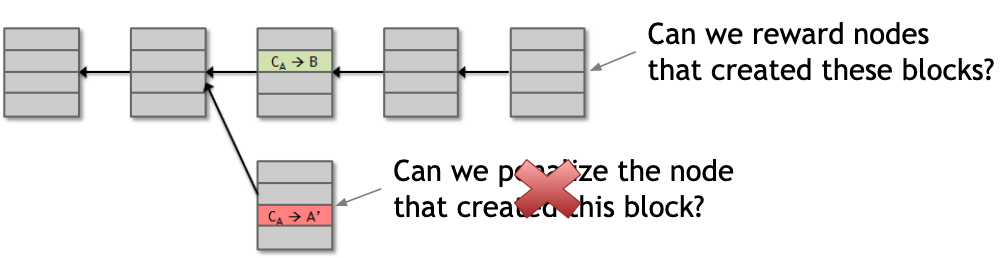
\includegraphics[scale=0.7]{incentives}

\end{frame}

%%%%%%%%%%%% Slide %%%%%%%%%%%%%%%%%%%%%%%%%%%%%%%%%%%%%%%%%%%%%%%%%%%
%\begin{frame}
%  \frametitle{CPU Mining Pseudocode}
%  \centering
%	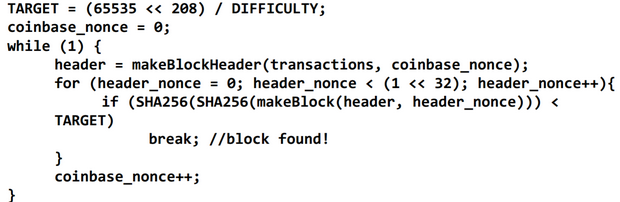
\includegraphics[scale=1.1]{mining}

%\end{frame}
%%%%%%%%%%%% Slide %%%%%%%%%%%%%%%%%%%%%%%%%%%%%%%%%%%%%%%%%%%%%%%%%%%
\begin{frame}
  \frametitle{Proof of Work Properties}
       \begin{block}{\textcolor{brown}{ Property 1: Difficult to compute.}}
       Only some nodes bother to compete - miners.
 	\end{block} 

	\pause
	
	\begin{block}{\textcolor{brown}{ Property 2: Parameterizable cost.}}
       Nodes automatically re-calculate the target every two weeks. \\
       \pause
       
Goal: \emph{average} time between blocks = 10 minutes

 	\end{block} 
 	
 	\pause
 	
 		\begin{block}{\textcolor{brown}{ Property 3: Trivial to verify.}}
       
Nonce must be published as part of block. \\


Other miners simply verify that
$H(nonce ‖ prev_hash ‖ tx ‖ … ‖ tx) < target$

 	\end{block} 
\end{frame}
%%%%%%%%%%%% Slide %%%%%%%%%%%%%%%%%%%%%%%%%%%%%%%%%%%%%%%%%%%%%%%%%%%
\begin{frame}
  \frametitle{Summary}
  Bitcoin has three types of consensus: 
	\begin{enumerate}
		\item Value
		\item State
		\item Rules
	\end{enumerate}
	\pause
  Next time:
	\begin{itemize}
		\item How do we get from consensus to currency?
		\item What else can we do with consensus?
    \end{itemize}		
\end{frame}
%%%%%%%%%%%% Slide %%%%%%%%%%%%%%%%%%%%%%%%%%%%%%%%%%%%%%%%%%%%%%%%%%%
\end{document}
